\documentclass{amsart}
\usepackage{amsmath}
\usepackage{amsfonts}
\usepackage{amssymb}
\usepackage{amsthm}
\usepackage{color,hyperref}
\usepackage[table,usenames,dvipsnames]{xcolor}
\usepackage{tikz}
\usetikzlibrary{matrix,arrows,positioning,automata}
\pgfdeclarelayer{background layer}
\pgfsetlayers{background layer,main}

\definecolor{darkblue}{rgb}{0.0,0.0,0.3}
\definecolor{lgr}{rgb}{0.9,0.9,0.9}
\definecolor{dgr}{rgb}{0.6,0.6,0.6}
\hypersetup{colorlinks,breaklinks,
            linkcolor=darkblue,urlcolor=darkblue,
            anchorcolor=darkblue,citecolor=darkblue}

\usepackage[norelsize,ruled,vlined,linesnumbered]{algorithm2e}

\newcommand{\cT}{{\mathcal T}}
\newcommand{\cS}{{\mathcal S}}
\newcommand{\Sub}{\mathbf{Sub}}
\newcommand{\Set}{\mathbf{Set}}
\newcommand{\Pos}{\mathbf{Pos}}
\newcommand{\Max}{\mathbf{Max}}
\newcommand{\compl}{\mathsf{c}}

\DeclareMathOperator{\Aut}{Aut}

\newcommand{\todo}[1]{ \small \textsf{[TODO:  #1 ]} \normalsize}


\theoremstyle{plain}
\newtheorem{theorem}{Theorem}[section]
\newtheorem{lemma}[theorem]{Lemma}
\newtheorem{fact}[theorem]{Fact}
\newtheorem{Proposition}[theorem]{Proposition}
\newtheorem{cor}[theorem]{Corollary}
\theoremstyle{definition}
\newtheorem{definition}[theorem]{Definition}
\newtheorem{example}[theorem]{Example}

\newcommand{\SgpDec}{\textsc{SgpDec}}
\newcommand{\GAP}{\textsc{Gap}}
\newcommand{\Viz}{\textsc{Viz}}
\newcommand{\GraphViz}{\textsc{GraphViz}}



\begin{document}
\title{On Enumerating Transformation Semigroups}
\author{James East$^1$ and Attila Egri-Nagy$^{1}$ and James D. Mitchell$^2$}
\address{$^1$Centre for Research in Mathematics, School of Computing, Engineering and Mathematics, University of Western Sydney (Parramatta Campus), Locked Bag 1797, Penrith, NSW 2751, Australia}
\address{$^2$ Mathematical Institute, University of St Andrews, North Haugh, St Andrews, Fife, KY16 9SS, Scotland}
\email{J.East@uws.edu.au,\ A.Egri-Nagy@uws.edu.au,\ jdm3@st-and.ac.uk}

\maketitle

\tableofcontents
\section{Introduction}
Previous efforts for enumerating semigroups were focused on the abstract case, enumerating by the order, and worked by finding all valid multiplication tables of the given size \cite{monoidenum2009}.
Here we enumerate transformation semigroups by degree.
For degree $n$ this is the task of enumerating all valid subtables inside one big multiplication table of the  full transformation semigroups $\cT_n$.

\section{Notation}
%Let $(X,S)$ be a transformation semigroup, $n=|S|$.
Let $S$ be finite a semigroup, $n=|S|$.
We fix an order on the semigroup elements $s_1,\ldots, s_n$, so we can easily refer to the elements by their indices. 
Then the  \emph{multiplication table}, or \emph{Cayley-table} of $S$ is a $n\times n$ matrix $M(S)$ or simply $M$ with entries from $\{1,..,n\}$ such that $M_{i,j}=k$ if $s_is_j=s_k$.
$M_A$ denotes the subarray of $M$ spanned by $A\subseteq\{1,\ldots,n\}$.
$R_i$ is the $i$th row and $C_j$ is the $j$th column vector of $M$.
We denote the set of the elements of a vector $v$ by $\Set(v)=\{x\mid x\in v\}$.
$\Pos(v,i)$ is the set of positions in vector $v$ containing the value $i$.

$\Sub(S)=\big\{T\mid T\leq S \big\}$ the set of all subsemigroups, $\Max(S)$ the set of maximal proper subsemigroups.
If $I$ is an ideal of $S$ then the \emph{Rees factor semigroup} $S/I$ has elements $S\setminus I\cup\{0\}$ with multiplication same as in $S$ if the product stays in $S\setminus I$ and zero otherwise.

$\cS_n$ denotes the symmetric group, $\cT_n$ the full transformation group on $n$ points.
\section{Useful facts}
We can simplify and parallelize enumerating subsemigroups by enumerating subsemigroups of its maximal subsemigroups and merge the results.
\begin{fact}
$\Sub(S)=\big( \bigcup_{T\in \Max(S)}\Sub(T)\big)\cup \{S\}$
\end{fact}
%\proof
%It follows from the fact that $\Sub(S)$ is an algebraic lattice.
%\qed

Once a subsemigroup is found, we can generate its conjugate subsemigroups.
\begin{fact}
$T\in\Sub(S)$ and $g\in \Aut(S)$ then $T^g\in\Sub(S)$.%$g^{-1}Tg\in\Sub(S)$.
\end{fact}
%\proof
%Let $s,t\in T$ and $T'=g^{-1}Tg$.
%$$g^{-1}sgg^{-1}tg=g^{-1}stg.$$
%\qed


Enumeration is truly parallel for an ideal and its corresponding factor semigroup followed by combining the results.
\begin{lemma}
Let $I$ be an ideal of $S$, then $$\Sub(S)=\big\{\langle (T\setminus\{0\})\cup U \rangle\mid T\in \Sub(S/I), U\in\Sub(I)\big\}.$$
\end{lemma}
\proof

\qed

\section{Multiplication Table Algorithms}

\subsection{Closure Algorithms}
Given a subsemigroup $T\leq S$ and a set of elements  $A\subseteq S$, the \emph{closure} of $T$ by $A$ is $\langle T\cup A \rangle$.
For calculating what subsemigroup a set $A$ generates, we can take the closure of $\varnothing$ by $A$, which is simply $\langle A\rangle$.

\subsubsection{Simple Method}
Checking $M_{T\cup A}$ for set of elements $B$ not in $T\cup A$. Then iterate with $T\cup A\cup B$.
\subsubsection{Global Tables}
Starting from the result of a product, we ask how can we produce element $k$?
All possible $s_is_j=s_k$ or $s_js_i=s_k$.
Thus the  answer is all $i,j$ coordinate pairs containing $k$, and in general these may be distributed all over the multiplication table $M$.
From the point of calculating the closure we can  omit coordinate pairs $i,j$ where $i=k$ of $j=k$. 
We do not need the order information, so we can talk about ordered pairs $(i,j)$, $i\leq j$. 
Let's denote the set of these pairs by $P_k$.

The set $P_k$ of all coordinate pairs encoding the locations is still redundant in a sense that instead of storing all pairs including $i$, we can simply record $i$ and all the other elements in those pairs.
For instance $(i,j)$ and $(i,h)$ can be stored as $(i,\{h,j\})$, therefore $i$ is only checked once.
Then the  global information table of $k$ is defined by
$$G_k=\bigcup_{(i,j)\in P_k} \left\{ (i,\{j\mid i\leq j\})\right\}.$$
These tables are useful when we would like to calculate the closure of a set $A$ which is relatively big in $S$.
We take $A\subseteq S$ and for all elements $k$ in $S\setminus A$ we check whether $G_k$ contains pairs from $X$ to decide whether $k$ is in $\langle A\rangle$ or not. 

\subsubsection{Local Tables} Given that we have a set elements $A\subseteq S$, what do we need to add when including a new element $i$?
%from the value, get the positions (value, positions) pairs
In particular, do we have to include an element $k$? The answer is by checking the positions. 

Let $V_i=\Set(R_i)\cup\Set(C_i)$, the values in generated by $i$. Then the  local information table for element $i$ is defined by
$$L_i=\bigcup_{k\in V_i}\left\{(k,\Pos(R_i,k)\cup\Pos(C_i,k))\right\}.$$
For instance if $(k,\{j,h\})\in L_i$ then either $s_is_j=s_k$ or $s_js_i=s_k$ and similarly for $h$.
When  extending $X\subseteq S$ by $i$, we check $L_i$ for each value $k$ not in $X$ whether its positions contain some elements from $X$. 
\subsection{Isomorphism and Anti-Isomorphism of Multiplication Tables}
Two semigroups $S$ and $T$ are isomorphic or anti-isomorphic if $M(S)$ can be transformed into $M(T)$ by rearranging its columns and rows and transposing the table.
By computing some global properties of the multiplication tables that are invariant under these rearrangings in some cases we can easily decide non-isomoprhism.
%These are the \emph{table level invariants}.
If all invariants check out, then we can use backtrack to find out whether one of the multiplication tables can be rearranged to get the other one.
An element of $C_2\times S_n$ can witness the isomorphism.
Fortunately we do not have to search through the whole symmetric group, we only need to consider some special permutations that take an element to another one with the same type.
Type is defined by the following invariants.
The search space can be reduced by aligning elements with the same profile (frequency, diagonal frequency, index-period).

\subsubsection{Element Types}

\begin{enumerate}
\item Frequency: the number of occurences of the element in the table.
\item Diagonal frequency: the number of occurences of the element in the diagonal of the table.
\item Index-period: the smallest values $m\geq 1$, $r\geq 1$ such that $a^{m+r}=a^m$.
\item Row and column partition: encoding how many distinct elements are in the right and left principal ideals and what are their frequencies.
\end{enumerate} 

\subsubsection{Table Invariants}

Any property that does not contain information about the ordering of the elements can be used as an invariant.
\begin{enumerate}
\item Distinct frequency values of elements in the table and the number of elements with a given frequency. Useless for groups as their multiplication tables are Latin squares.
\item Column and row partitions types.   Useless for groups since all the principal ideals are the same.
\item The diagonal partition. $|S|=n$ partitioned as a sum of number of occurences of elements in the diagonal. This can even tell some groups apart: $C_4\mapsto 2+2$, $C_2\times C_2\mapsto 4$, but it assings 2+6 to both $D_8$ and $Q_8$.
\item Distinct composite element types: putting together all the element types. In the group case this invariant reduces to the order of elements, but it can distinguish between $D_8$ and $Q_8$. However, this invariant fails to detect the difference between some direct and semidirect products. For instance, $C_8\times C_2$ and $C_8\rtimes C_2$ both have 1 element of order 1, 3 of order 2, 4 of order 4, and 8 of order 8.
\end{enumerate} 







\section{Subsemigroup Enumeration Algorithms}

\subsection{Enumerating by 1-extensions}

\begin{algorithm}
\SetKwInOut{Input}{input}\SetKwInOut{Output}{output}
\SetKwData{subs}{subs}
\SetKwData{diff}{diff}
\SetKwFunction{Extend}{Extend}
\Input{$S$ semigroup, $T\leq S$,\subs, $s\in S$ }
\Output{\subs with all possible extensions of $T$ added}
\SetKwInOut{Name}{\Extend($T$,$s$,$S$,\subs)}
\BlankLine
\Name{}

$T'$ $\leftarrow$ $\langle T\cup\{s\}\rangle$\\
    \If{$T'\notin$ \subs}{
      \subs$\leftarrow$ \subs$\cup\{T'\}$\\
      \diff $\leftarrow$ $S\setminus T'$\\
      \For{$t\in$\diff}{
      \Extend($T',t,S$,\subs)
    }
  }
\caption{Finding all subsemigroup containing $T$ in $S$ .\textsf{subs} $\leftarrow$ $\varnothing$ $s\in S$ \textsf{Extend}($\varnothing,s,S$,\textsf{subs}) enumerates all subsemigroups of $S$.}
\label{alg:1-extensons}
\end{algorithm}

\subsection{Parallel Enumeration in Ideal Quotients}

\section{Enumerating transformation semigroups of degree 2,3 and 4}

\subsection{$\cT_2$, The Pen and Paper Case}
Since $\cT_2$ has only four elements, thus the search space size is only $2^4=16$, it is an easy exercise to find all of its subsemigroups. 
Using one-line notation for permutations, we order the elements lexicographically, 1=[1,1], 2=[1,2], 3=[2,1], 4=[2,2]. Here are the closed subarrays.
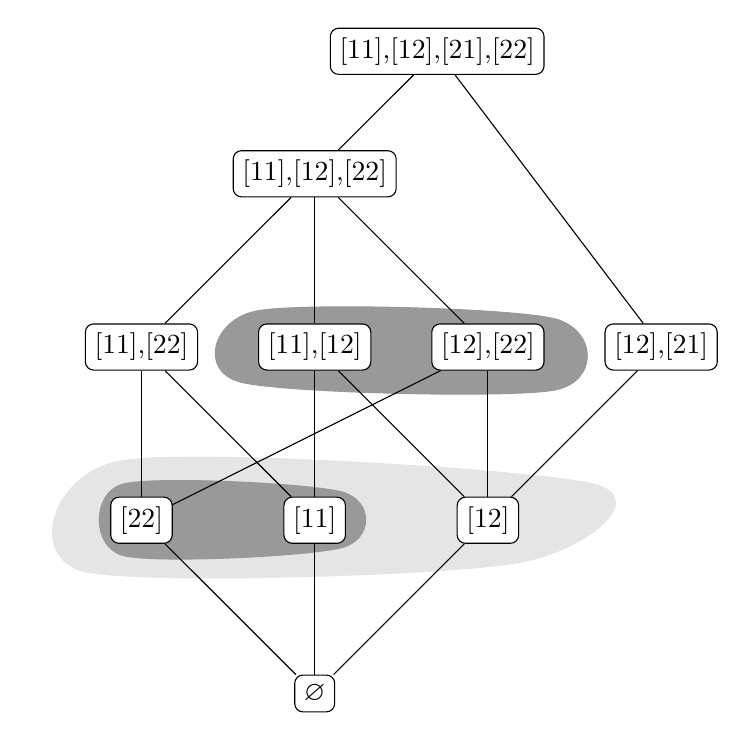
\begin{tikzpicture}
[align=center,node distance=2.2cm]
\tikzstyle{plain}=[fill=white,rounded corners=3pt, draw]

\draw node [plain] (1234) {[11],[12],[21],[22]};
\draw node [plain,below left of=1234] (124) {[11],[12],[22]};
\draw node [plain,below of=124] (12) {[11],[12]};
\draw node [plain,left of=12] (14) {[11],[22]};
\draw node [plain,right of=12] (24) {[12],[22]};
\draw node [plain,right of=24] (23) {[12],[21]};

\draw node [plain,below of=12] (1) {[11]};
\draw node [plain,left of=1] (4) {[22]};
\draw node [plain,right of=1] (2) {[12]};
\draw node [plain,below of=1] (empty) {$\varnothing$};

\draw  (1234) -- (124);
\draw (124) -- (12);
\draw (124) -- (24);
\draw (124) -- (14);
\draw  (1234) -- (23);
\path (23) edge (2);
\draw (1) -- (empty);
\draw (2) -- (empty);
\draw (4) -- (empty);
\draw (14) -- (4);
\draw (14) -- (1);
\draw (12) -- (2);
\draw (12) -- (1);
\draw (24) -- (4);
\draw (24) -- (2);
\begin{pgfonlayer}{background layer}
\filldraw [dgr] plot [smooth cycle] coordinates {(1.5,-4.3)(-2.5,-4.2) (-2.3,-3.3) (1.5,-3.4)};
\filldraw [lgr] plot [smooth cycle] coordinates {(-4,-5.2) (2,-5.5) (1,-6.5)(-4.5,-6.6)};
\filldraw [dgr] plot [smooth cycle] coordinates {(-4,-5.5) (-1.2,-5.6) (-1.2,-6.3)(-4,-6.4)};
\end{pgfonlayer}

\end{tikzpicture}
Using these we can draw the subsemigroup lattice (Fig.\ \ref{fig:T2subs}).

\begin{figure}
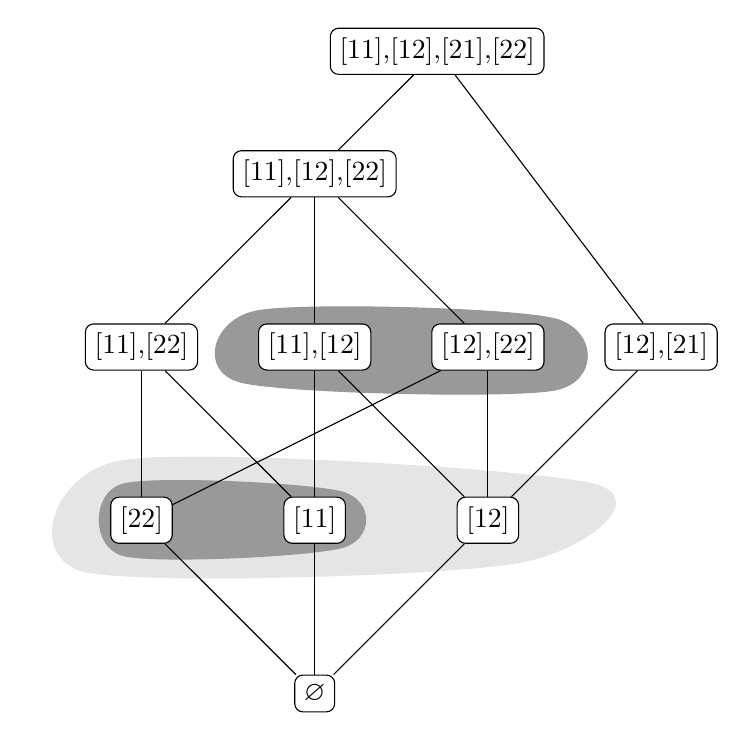
\begin{tikzpicture}
[align=center,node distance=2.2cm]
\tikzstyle{plain}=[fill=white,rounded corners=3pt, draw]

\draw node [plain] (1234) {[11],[12],[21],[22]};
\draw node [plain,below left of=1234] (124) {[11],[12],[22]};
\draw node [plain,below of=124] (12) {[11],[12]};
\draw node [plain,left of=12] (14) {[11],[22]};
\draw node [plain,right of=12] (24) {[12],[22]};
\draw node [plain,right of=24] (23) {[12],[21]};

\draw node [plain,below of=12] (1) {[11]};
\draw node [plain,left of=1] (4) {[22]};
\draw node [plain,right of=1] (2) {[12]};
\draw node [plain,below of=1] (empty) {$\varnothing$};

\draw  (1234) -- (124);
\draw (124) -- (12);
\draw (124) -- (24);
\draw (124) -- (14);
\draw  (1234) -- (23);
\path (23) edge (2);
\draw (1) -- (empty);
\draw (2) -- (empty);
\draw (4) -- (empty);
\draw (14) -- (4);
\draw (14) -- (1);
\draw (12) -- (2);
\draw (12) -- (1);
\draw (24) -- (4);
\draw (24) -- (2);
\begin{pgfonlayer}{background layer}
\filldraw [dgr] plot [smooth cycle] coordinates {(1.5,-4.3)(-2.5,-4.2) (-2.3,-3.3) (1.5,-3.4)};
\filldraw [lgr] plot [smooth cycle] coordinates {(-4,-5.2) (2,-5.5) (1,-6.5)(-4.5,-6.6)};
\filldraw [dgr] plot [smooth cycle] coordinates {(-4,-5.5) (-1.2,-5.6) (-1.2,-6.3)(-4,-6.4)};
\end{pgfonlayer}

\end{tikzpicture}
\caption{$\Sub(\cT_2)$, dark grey blobs indicate nontrivial conjugacy classes, light grey shows an isomorphism class.}
\label{fig:T2subs}
\end{figure}
\todo{explain frequencies of elements in multiplication table}


\begin{table}
\renewcommand{\arraystretch}{1}
\begin{tabular}{|c|r|r|r||r|r|r||r|r|r|}
\hline
$K_{i,j}$ & \multicolumn{3}{c||}{$j=1$} & \multicolumn{3}{c||}{2} & \multicolumn{3}{c|}{3} \\
\hline
$i=2$ & 4&3&3   & \cellcolor{lgr}  & \cellcolor{lgr}&  \cellcolor{lgr} & \cellcolor{lgr}  &\cellcolor{lgr} &\cellcolor{lgr}\\
\hline
$3$ &  8&4&4  &  600 & 123 & 118  & \cellcolor{lgr}  & \cellcolor{lgr}&\cellcolor{lgr}\\
\hline
$4$ & 16&5&5  &   & 162332 &   &   & &\\
\hline
$n$ & $2^n$&$n+1$&$n+1$    &    & &    &    & & \\
\hline

\end{tabular}
\caption{Number of subsemigroups of ideals in of full transformation semigroups. The second and third numbers are the number of distinct subsemigroups up to conjugacy and isomorphism.}
\end{table}


\begin{table}
\renewcommand{\arraystretch}{1}
\begin{tabular}{|c|r|r|r|}
\hline
 & \#subsemigroups & \#conjugacy classes & \#isomorphism classes \\
\hline
$\cT_0$ & 1  & 1 & 1\\
\hline
$\cT_1$ & 2  & 2 & 2\\
\hline
$\cT_2$ & 10  & 8 & 7\\
\hline
$\cT_3$ & 1299 & 283 & 267\\
\hline
%$\cT_4$ & & & \\
%\hline
\end{tabular}
\caption{Number of subsemigroups of full transformation semigroups.}
\end{table}

\bibliography{subsemi}
\bibliographystyle{plain}

\end{document}